\clearpage

\section{에이전트와 C2 통신}\label{sec:c2}

\subsection{비컨 주기와 명령 전달}\label{subsec:beacon}

에이전트는 설정된 비컨 간격에 따라 C2 서버에 주기적으로 접속한다. 이 접속을 \textbf{비컨}이라 한다.
에이전트와 C2 사이의 통신은 명령을 수신하기 위한 \textbf{정기 비컨}과 실행 결과를 전송하기 위한 \textbf{결과 보고}로 구분된다(그림~\ref{fig:beacon}).
두 요청은 C2 서버의 동일한 접속 경로를 사용하지만, 요청 데이터의 구성과 처리 방식은 서로 다르다.

정기 비컨 한 주기에는 다음 절차가 순서대로 진행된다.

\begin{enumerate}
    \item 에이전트가 자신의 정보(호스트 이름, 사용자, 플랫폼, 아키텍처, 권한, 지원하는 셸 목록, 프로세스 ID(PID) 등)를 전송한다. 정기 비컨에는 실행 결과가 포함되지 않는다.
    \item C2는 최초로 접속한 에이전트에 고유 식별자(Paw)를 부여하여 등록하고, 이미 등록된 에이전트의 경우 에이전트 정보와 최근 접속 시각을 갱신한다.
    \item 해당 에이전트에 배정된 `대기' 명령을 모두 조회한 뒤 상태를 `전송됨'으로 변경하고 응답에 포함한다.
    \item 다음 비컨까지의 대기 시간을 함께 전달한다. 대기 시간은 비컨 최소·최대 간격 범위에서 무작위로 결정하여 접속 간격이 일정해지지 않도록 한다.
\end{enumerate}

에이전트는 수신한 명령을 각각 실행하고, 각 명령의 실행이 완료될 때마다 다음 정기 비컨을 기다리지 않고 즉시 결과 보고를 전송한다.
결과 보고에는 실행 결과와 함께 에이전트 정보 중 일부(식별자, 호스트, 플랫폼, 접속 주소)만 포함된다.
C2는 결과 보고를 다음과 같이 처리한다.

\begin{enumerate}
    \item 실행 결과를 저장하고 해당 명령의 상태를 `완료'로 변경한다. 해당 명령이 공격 실행 단계에 해당하는 경우 엔진이 다음 단계를 대기열에 등록한다(\ref{sec:operations}장).
    \item 에이전트 정보는 결과 보고에 실제로 포함된 항목만 갱신하고, 나머지 항목(셸 목록, 그룹, 사용자 등)은 기존 값을 유지한다.
    \item 에이전트는 결과 보고에 대한 응답을 처리하지 않으므로, 응답에 대기 명령을 포함하지 않는다. 새로 등록된 명령은 다음 정기 비컨에서 전달된다.
\end{enumerate}

\begin{figure}[H]
\centering
\begin{tikzpicture}[every node/.style={font=\footnotesize}]
  \node[box, minimum width=24mm] (con) at (0,0) {운영 콘솔};
  \node[box, minimum width=24mm] (db)  at (4.2,0) {공유 데이터베이스};
  \node[hot, minimum width=24mm] (c2)  at (8.4,0) {C2 서버};
  \node[ext, minimum width=24mm] (ag)  at (12.6,0) {에이전트};
  \foreach \n in {con,db,c2,ag} \draw[ksgray, densely dotted] (\n.south) -- ++(0,-6.6);

  \draw[arr] (0,-0.9) -- node[lbl, above]{명령 기록(대기)} (4.2,-0.9);
  \draw[arr] (12.6,-1.7) -- node[lbl, above]{정기 비컨: 에이전트 정보} (8.4,-1.7);
  \draw[arr] (4.2,-2.4) -- node[lbl, above]{대기 명령 → 전송됨} (8.4,-2.4);
  \draw[arr] (8.4,-3.1) -- node[lbl, above]{명령 목록 + 대기 시간} (12.6,-3.1);
  \node[lbl, anchor=west, fill=white, inner sep=1pt] at (12.75,-3.8) {실행};
  \draw[arr] (12.6,-4.6) -- node[lbl, above]{결과 보고: 일부 정보 + 결과} (8.4,-4.6);
  \draw[arr] (8.4,-5.3) -- node[lbl, above]{결과 저장 · 다음 단계 등록} (4.2,-5.3);
  \draw[arr] (4.2,-6.0) -- node[lbl, above]{결과 조회} (0,-6.0);
\end{tikzpicture}
\caption{정기 비컨과 결과 보고의 흐름}
\label{fig:beacon}
\end{figure}

명령 본문과 결과는 에이전트가 요구하는 메시지 형식(명령 목록을 별도로 인코딩하여 인코딩된 메시지에 포함하는 구조)을 따른다.
에이전트는 응답의 필수 항목이 하나라도 빠지면 별도의 오류 메시지 없이 비정상 종료하므로, C2 서버는 응답 메시지에 모든 필수 항목을 포함한다.

\subsection{에이전트 배포}\label{subsec:deploy}

에이전트 화면에서 `에이전트 배포'를 클릭하면 대상 플랫폼별 설치 명령이 표시된다(그림~\ref{fig:deploy}).
운영자가 `C2 주소'와 `임플란트 이름'을 변경하면 표시된 설치 명령이 입력값에 따라 즉시 갱신된다.
대상 호스트에서 설치 명령을 실행하면 다음 절차가 수행된다.

\begin{itemize}
    \item 대상 호스트의 아키텍처를 확인한 후, C2에서 그에 맞는 에이전트 바이너리를 내려받는다. C2 서버는 요청에 포함된 플랫폼 및 아키텍처 정보를 기반으로 사전에 빌드된 바이너리 중 적합한 파일을 제공한다.
    \item 내려받은 파일은 운영자가 정한 임플란트 이름으로 저장된다. 정상 프로세스와 유사한 이름을 지정하여 방어 제품이 프로세스 이름만으로 에이전트를 식별하는지 확인하기 위한 것이다.
    \item 에이전트는 C2 주소와 그룹(기본값: red)을 실행 인자로 전달받으며, 최초 비컨을 통해 등록된다. 배포 화면에서는 새 에이전트의 접속을 대기하고, 연결이 완료되면 접속 상태를 표시한다.
\end{itemize}

추가 배포 방식(`변형')으로는 blue 그룹 등록과 임의의 이름으로 파일을 내려받아 백그라운드 프로세스로 실행하는 방식 등이 있다.
명령 실행 도구를 사용할 수 없는 호스트를 위해 에이전트 바이너리를 직접 내려받는 `바이너리 다운로드' 기능도 제공한다.
`설정' 탭에서는 모든 에이전트에 적용되는 비컨 최소·최대 간격, 워치독 및 비신뢰 타이머를 설정할 수 있다.
비컨 간격을 변경하면 기존에 접속한 에이전트에도 다음 비컨부터 변경된 설정값이 적용된다.

\begin{figure}[H]
\centering
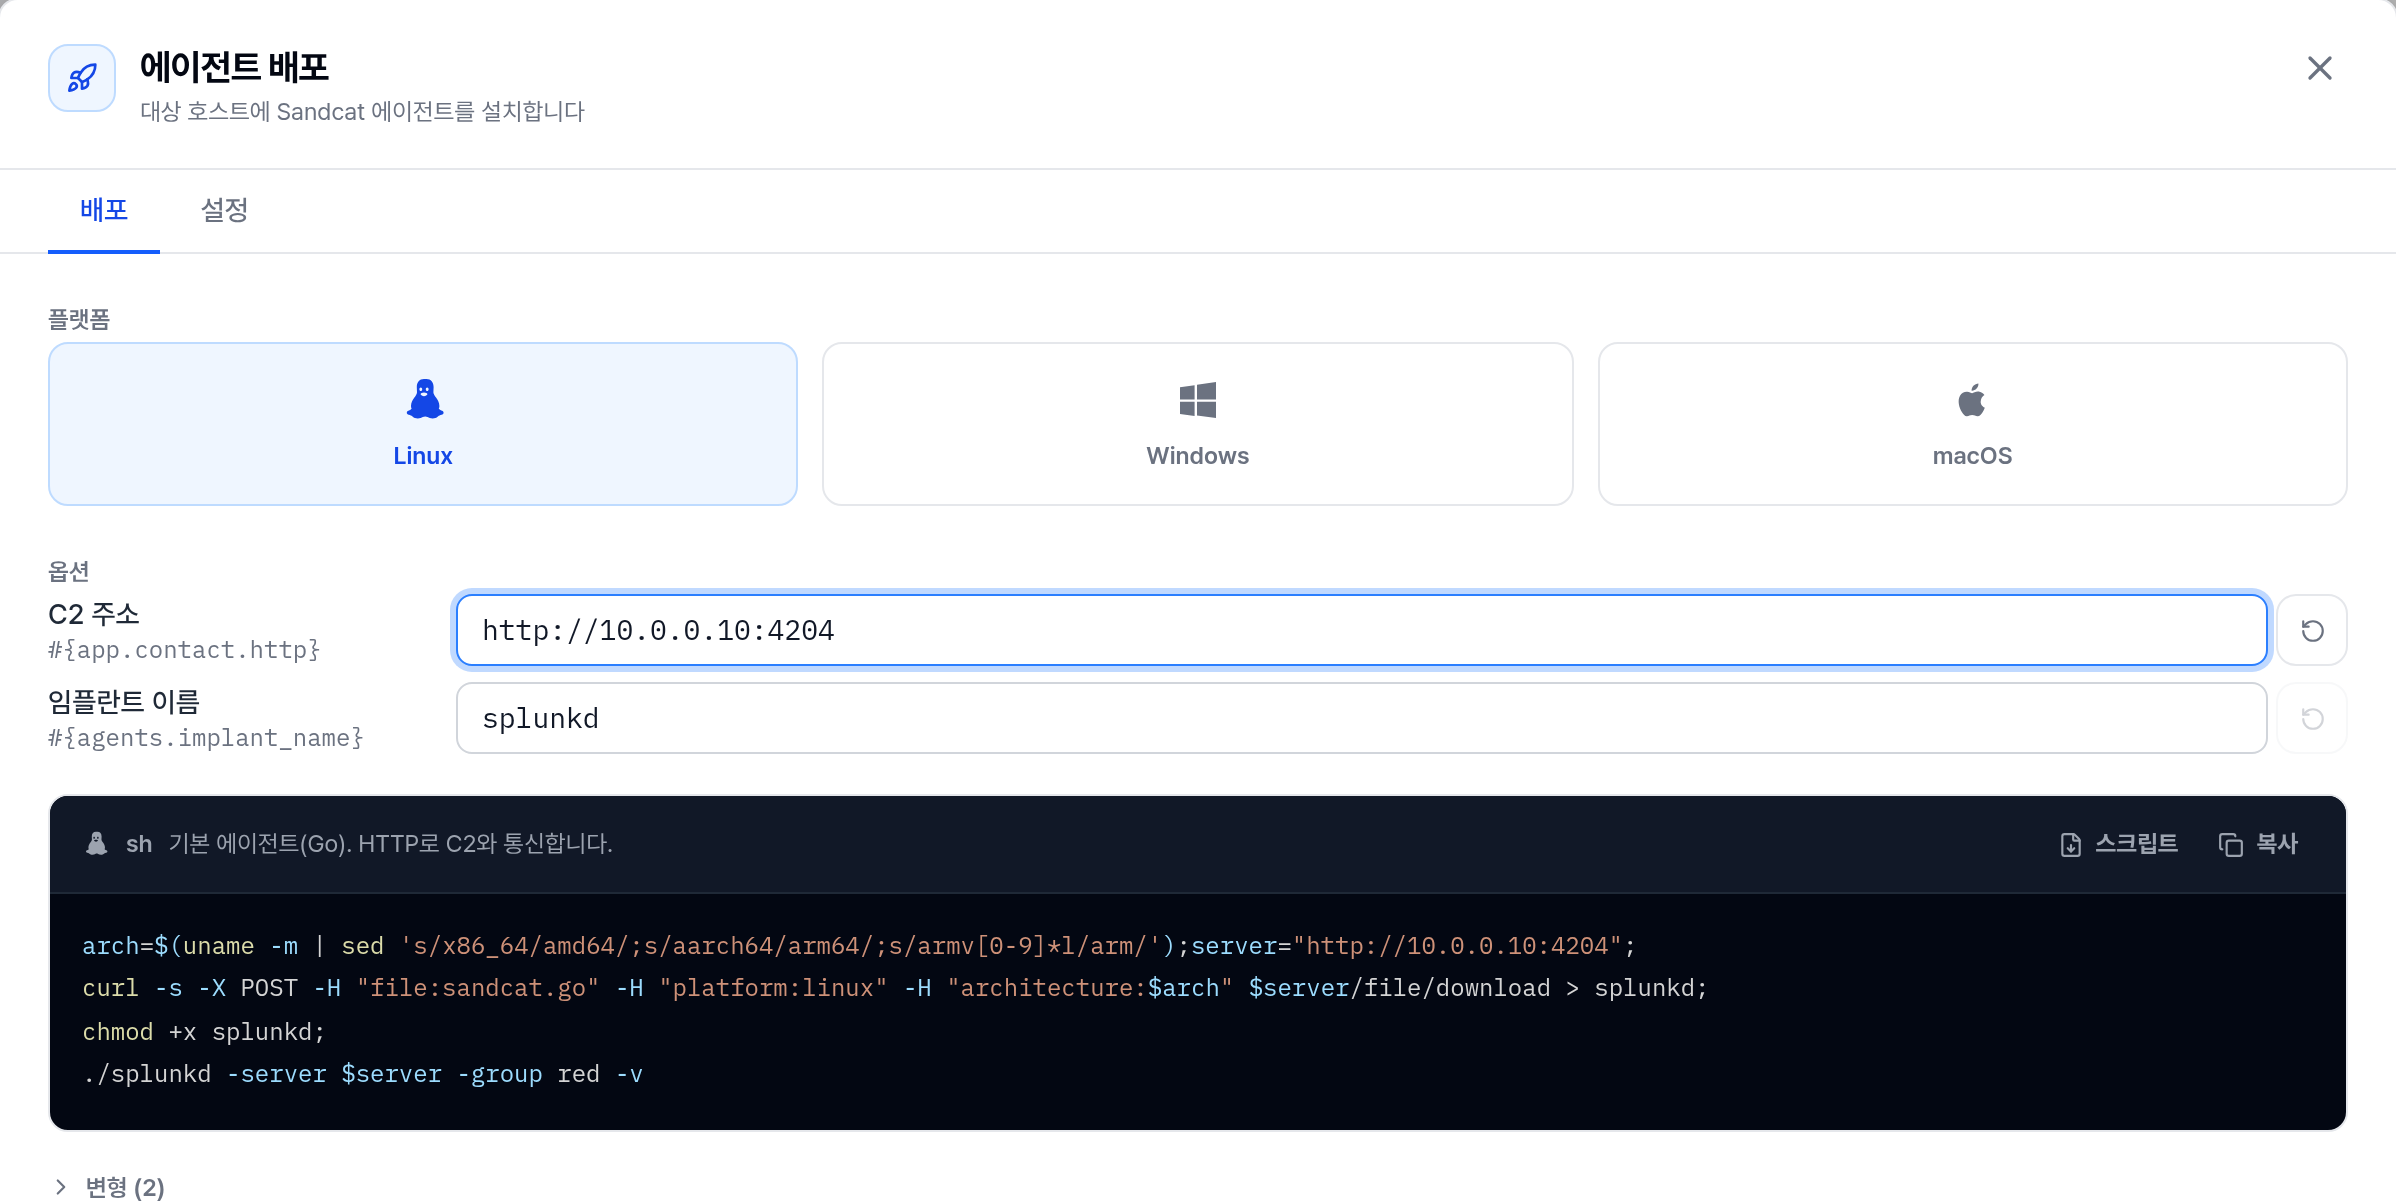
\includegraphics[width=0.62\textwidth]{screenshots-bas/deploy.png}
\caption{에이전트 배포 창(Linux 기본 설치 명령)}
\label{fig:deploy}
\end{figure}

\subsection{에이전트 상태 판단}\label{subsec:trust}

에이전트는 별도의 생존 상태 신호를 전송하지 않는다. 플랫폼은 마지막 비컨 이후의 경과 시간을 기준으로 에이전트 상태를 판단한다.
경과 시간이 `비신뢰 타이머' 설정값(기본 90초) 이내이면 `신뢰', 이를 초과하면 `비신뢰'로 표시한다.
대시보드의 신뢰·비신뢰 에이전트 수도 같은 기준으로 계산된다.

에이전트 목록에서 제공하는 `종료' 기능은 두 단계로 처리된다.
먼저 에이전트가 보고한 프로세스 ID(PID)를 이용해 자기 자신을 종료하는 명령을 대기열에 등록하고, 해당 명령의 결과를 최대 8초간 기다린다.
이후 운영 콘솔에서 해당 에이전트 정보와 명령 기록을 삭제한다.
에이전트는 지속성(재부팅 후 자동 실행) 기능이 없으므로 프로세스 종료 이후 자동으로 재실행되지 않는다.

\subsection{실시간 터미널}\label{subsec:terminal}

Pull 기반 명령 전달 방식에서는 에이전트가 다음 비컨을 전송할 때까지 명령 전달이 지연된다.
비컨 간격이 수십 초인 경우 대화형 명령 실행에 상당한 지연이 발생할 수 있다.
플랫폼은 \textbf{대화형 상태 유지 구간(window)}을 활용하여 이러한 지연을 줄인다.

\needspace{6\baselineskip}
운영자가 에이전트의 `터미널'을 열면, 콘솔은 약 5초마다 해당 에이전트의 터미널이 활성화되어 있음을 알리는 신호를 전송한다.
신호를 받을 때마다 해당 에이전트의 대화형 상태의 만료 시각이 신호 수신 시점으로부터 60초 후로 갱신되고, 이 상태가 유지되는 동안 C2는 비컨 응답에 다음 접속까지의 대기 시간을 1초로 설정하여 전달한다.
이에 따라 에이전트는 1초 간격으로 접속하게 되며, 터미널에 입력한 명령은 일반적으로 약 1초 이내에 에이전트에 전달된다.
터미널을 닫으면 대화형 상태가 해제되고, 이후 비컨부터 기존에 설정된 비컨 간격이 적용된다.

대화형 상태 유지 시간을 신호 전송 주기보다 충분히 길게 설정한 이유는 브라우저의 백그라운드 탭에서 타이머 실행이 지연되거나 네트워크 연결이 일시적으로 중단되어 일부 신호가 누락되더라도 대화형 상태가 해제되지 않도록 하기 위해서이다.
또 변경된 비컨 간격은 에이전트의 다음 비컨부터 적용되므로, 콘솔은 터미널 활성화 이후 에이전트의 비컨을 확인한 후 `세션 연결됨' 상태로 표시한다.
그전에도 명령 입력은 가능하지만, 기존 비컨 간격에 따라 명령 전달이 지연될 수 있음을 운영자에게 명확히 알리기 위한 것이다.

터미널 명령은 공격 실행과 같은 대기열을 사용한다.
명령은 에이전트가 실행되는 운영체제의 기본 셸(Windows는 PowerShell, 그 밖에는 sh)로 실행되며, 콘솔은 짧은 간격으로 결과 도착 여부를 확인하고, 결과가 수신되면 화면에 출력한다.
그림~\ref{fig:terminal}는 시험 호스트의 에이전트에 접속하여 사용자·계정·커널 정보를 조회한 화면이다.

\begin{figure}[H]
\centering
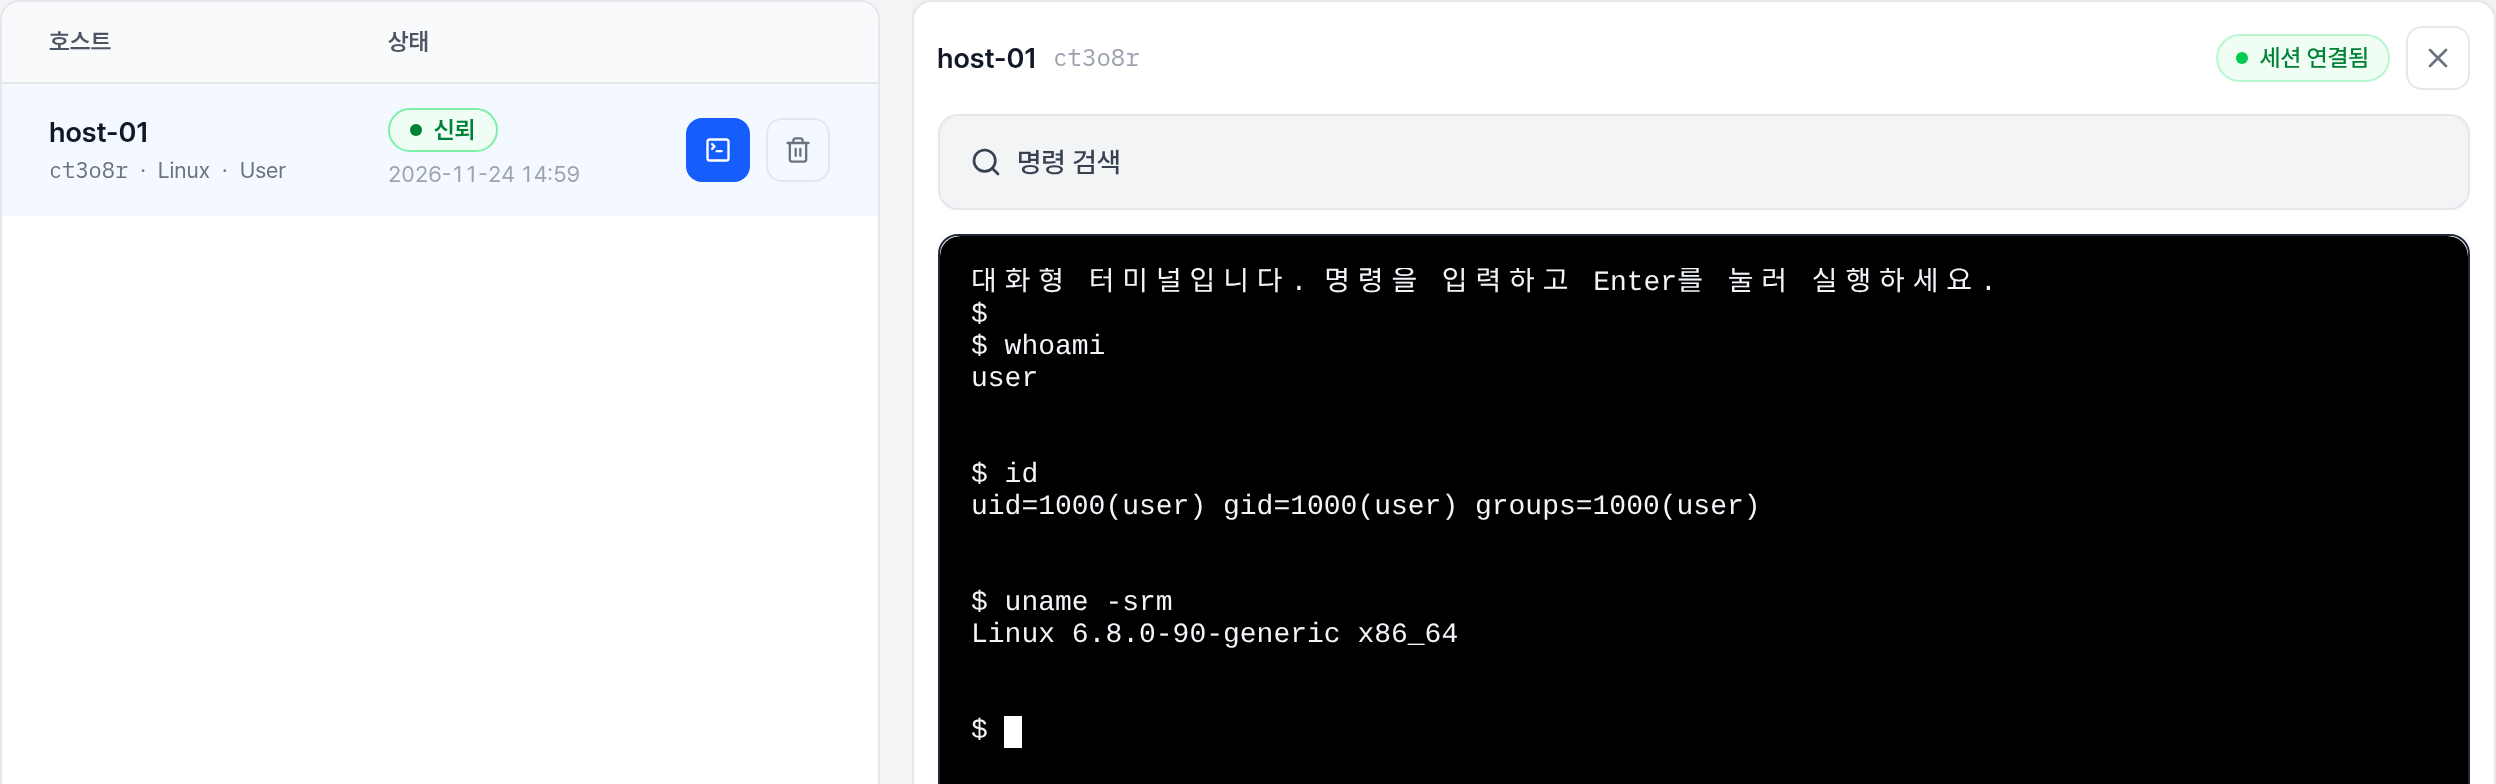
\includegraphics[width=0.72\textwidth]{screenshots-bas/terminal.png}
\caption{에이전트 터미널(시험 호스트에서 정보 조회 명령 실행)}
\label{fig:terminal}
\end{figure}

\subsection{페이로드와 파일 수집}\label{subsec:payload}

일부 Ability의 실행에는 명령문 외에도 별도의 실행 파일이나 스크립트(페이로드)가 필요하다.
에이전트는 해당 명령을 수신하면 먼저 C2에서 페이로드를 내려받은 뒤 명령을 실행한다.
C2는 운영자가 페이로드 보관 위치에 저장해 둔 파일만 제공하며, 요청된 파일명에서 경로 정보를 제거하여 지정된 보관 디렉터리 밖의 파일에 접근하지 못하도록 한다.
에이전트가 수집한 파일을 업로드하면 C2는 에이전트별로 구분된 위치에 저장한다.
